\documentclass[document.tex]{subfiles}
\begin{document}

\chapter{Feature Mining and Classification}
\section{Introduction}
\noindent Over the past few decade hyperspectral image sensor
has become one of the most powerful and fastest growing technologies in the field of remote sensing \cite{3}. Hyperspectral sensors collect land cover reflectance in many narrow contiguous spectral bands and form a large data cube\cite{3}. For instance, the hyperspectral imaging sensors like NASA Airborne Visible/Infrared Imaging
Spectrometer (AVIRIS) which simultaneously measures 224 bands with a fine resolution of 0.01 $\mu$m in the spectral range of visible to near infrared. This data cube contains rich information for wide range of application including effective land cover detection and classification \cite{24}. This large data also presents some challenges while classifying into constituent objects. A major classification challenge is when the training data set is small in compare to feature space dimensions, the classification starts to decrease. This problem is known as the curse of dimensionality or Hughes phenomenon\cite{4}\cite{25}\cite{26}. On the other hand, some bands are highly correlated and can be removed. In addition not all the bands are important for a specific classification problem. Therefore, an efficient and reliable technique to extract most informative and relevant features for classification is a major interest in current literature. The aforementioned feature reduction problem can be addressed using two basic approaches\cite{2}. One is the extraction of limited number of features after mapping to a new feature space based on some criteria like variance \cite{27,28}\cite{8}\cite{7}. For instance, PCA reduces the dimensionality of the input hyperspectral image which mitigates the curse of dimensionality. In PCA, an orthogonal transformation is performed to uncorrelate the input data set and the components are selected with higher variance. However, PCA doesn't consider the class structure of input data and depends solely on the global variance. Therefore, some noisy bands with high variance can be selected as a resultant feature. This limits the performance of PCA in classification task. An alternative approach to overcome the limitation of PCA and to find an effective subspace, some sorts of feature selection on PCA can be applied\cite{34}. Normalized Mutual Information (NMI) is one of the most popular feature selection technique\cite{9,10,20}.

\noindent Thus, feature extraction and feature selection gives a significant improvement in the classification accuracy. In some application of hyperspectral image only one class may be needed to identify at a time. For example, in land cover identification, if the objective is to identify forest land, we may not be interested in any other class except forest of the data set. In this paper, a target class oriented feature selection method is proposed which uses normalized mutual information measure over PCA data to maximize the relevance  of the input selected subset. Thus, feature selection over PCA based on target class samples also  overcomes the limitation of the PCA. Finally, the Kernel Support Vector Machine (KSVM) classifier is used to assess the effectiveness of the proposed method. 

\noindent Feature mining generally refers to transform a high dimensional correlated dataset into a low dimensional uncorrelated data space. It can be done by following two steps:
\begin{itemize}
	\item Feature extraction
	\item Feature selection
\end{itemize}

\section{Feature Extraction}
%\noindent Principal component analysis (PCA)\cite{7} is one of the most popular unsupervised feature extraction technique.The principal component analysis is based on the fact that neighboring bands of hyperspectral images are highly correlated and often convey almost the same information about the object. The PCA employs the statistic properties of
%hyperspectral bands to examine band dependency or correlation. This transformation
%is based on the mathematical principle known as eigenvalue decomposition of the
%covariance matrix of the hyperspectral image bands to be analyzed. The new transformed uncorrelated variables called principal components (PCs). First few variable contains most of the variation of the original data. If a hyperspectral image form M = i * j * k dataset where i is number of rows, j is number of columns and k is the number of bands of the dataset. Then after applying PCA to our dataset, we can use a small portion of k and still find almost all variations of our data. $X_1,X_2,X_3,....,X_n$ is the bands of the dataset. 
%\begin{comment}
%\begin{figure}[H]
%	\begin{center}
%		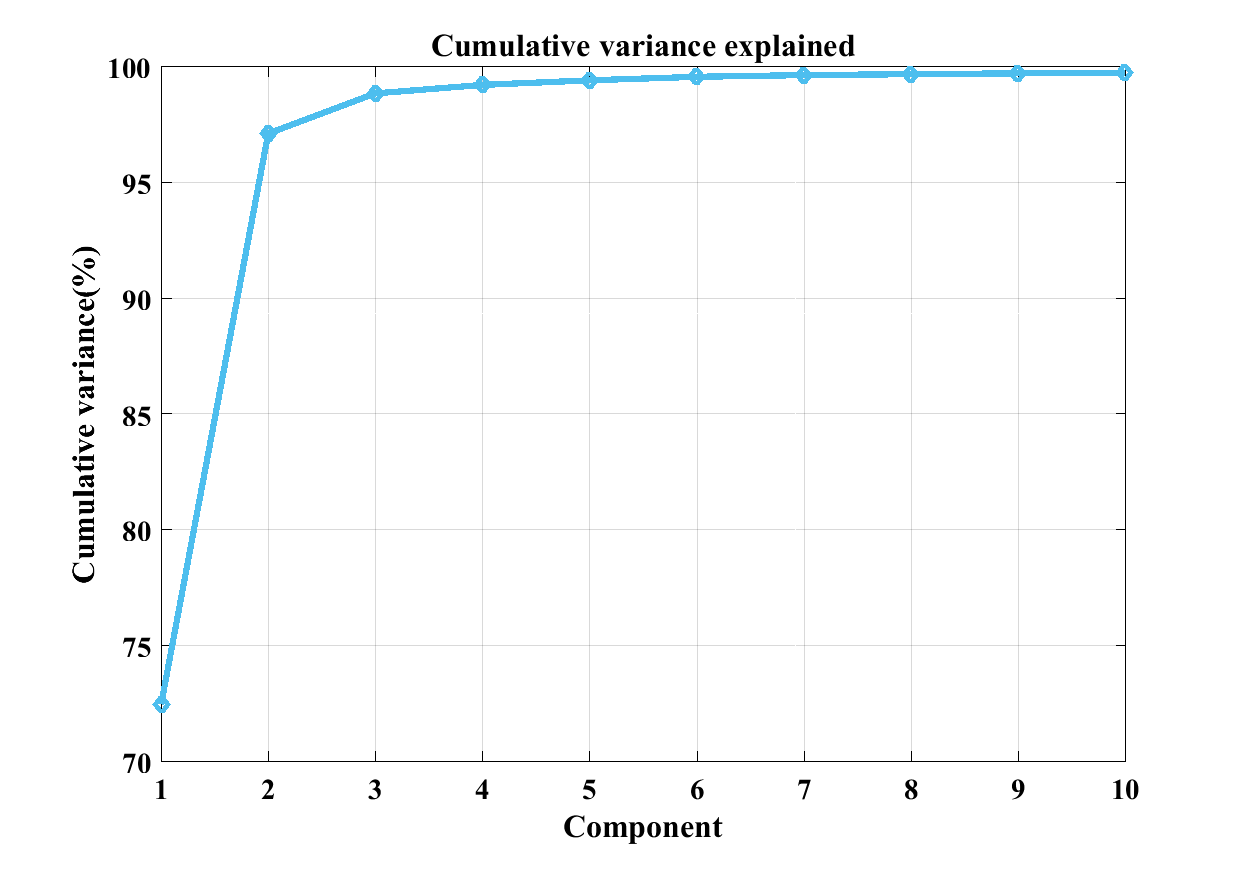
\includegraphics[height=8.0cm]{imgs/variance.png}
%	\end{center}
%	\caption{Cumulative variance of bands obtained via PCA}
%	\label{fig:Cumulative variance of bands obtained via PCA}
%\end{figure}
%\end{comment}
%\noindent For calculating PCA we first subtract mean form the dataset. The mean is calculated as
%\begin{equation}
%\overline{X} = \dfrac{\sum_{i=1}^{n} X_i}{n}
%\label{eq:Mean}
%\end{equation}
%The covariance matrix between any two dimension can be calculated as:
%\begin{equation}
%COV(X,Y) = \dfrac{\sum_{i=1}^{n}(X_i - \overline{X})(Y_i - \overline{Y})}{n-1}
%\end{equation}
%Covariance matrix is a square matrix. Eigenvalue and eigenvector is calculated from covariance matrix. Eigenvector that has the highest eigenvalue is the first principal component. Arrangement of eigenvectors according to descending order of eigenvalues creates a matrix of new set of data whose first few column can be chosen for further use.

Principal Component Analysis produces a new set of reduced and uncorrelated features. PCA works well on hyperspectral image as the neighboring bands of hyperspectral images are highly correlated and often convey similar information about the land cover object. PCA performs  the eigenvalue decomposition of covariance matrix of the input hyperspectral image. The new transformed uncorrelated images is called principal component (PCs). Let \textbf{X} be the input data cube and $\textbf{X}_1,\textbf{X}_2,...,\textbf{X}_n$ be the bands of the image. The covariance matrix is calculated as: 
\begin{equation}
cov(\textbf{X}_2,\textbf{X}_2) = \dfrac{\sum_{j=1}^{n}(X_1^j-\mu_1)(X_2^j-\mu_2)}{n}
\end{equation}

\noindent From this covariance matrix eigenvalue and eigenvector is determined. The eigenvectors are ordered according to the highest eigenvalue. This first few eigenvectors are selected as principal component as they contain most of the variance of the data set. The new features can be obtained as:
\begin{equation}
\textbf{Y} = \textbf{E}^T\textbf{X}
\end{equation}

\noindent Where \textbf{Y} is the transformed PCA data and $\textbf{E}^T$ is the matrix of normalized eigenvectors ordered by the higher eigenvalues. The first few components can be used as the extracted features.

 
\section{Feature Selection Based on Normalized Mutual Information}
%\noindent Mutual Information (MI) measures the amount of information one random variable holds about the other random variable\cite{20} by quantifying dependencies of those variables. Mutual information of two random varibles X and Y can be defined as:
%\begin{equation}
%I(X,Y) = \sum_{y=1}^{L1}\sum_{x=1}^{L2}p(x,y)\log\dfrac{p(x,y)}{p(x)p(y)}
%\end{equation}
%where x, y are the pixel values and L1, L2 are the maximum
%pixel values of the input images. P(x,y) is joint probability distribution function and P(x) and P(y) is marginal probability distribution function of variable X and Y respectively. If two variable x and
%y are independent, x does not know any information about y and vice versa. So their
%mutual information will be zero. According to Shannon’s information theory, if the
%probability of a random variable x is P(x) then uncertainty of x measured by entropy\cite{20} is:
%\begin{equation}
%H(x) = -p(x)log(p(x))
%\end{equation}
%Here mutual information can also be described as:
%\begin{equation}
%I(X,Y) = H(X) + H(Y) - H(X,Y)
%\end{equation}
%Where H(A) and H(B) are the entropies of A and B and H(A,B)
%is their joint entropy. Now by calculating mutual information between class label $c = c_1,c_2,....c_N$ and bands $f = f_1,f_2,...f_N$ of the hyperspectral image we can select relevant features for classification. Each feature will be selected in descending order $I_1 \geq I_2 \geq I_3 \geq....\geq I_N$. Feature with highest mutual information contains most information. It is difficult to use the value given by (4.3) directly in an absolute sense, as it is affected by the entropy of the two variables and not bounded to [0, 1]. A few methods to normalize mutual information are available to give a new value between 0 and 1, where 0 is the value for the independent case and 1 for the identical or one-to-one relationship case. Normalized mutual information (nMI)\cite{21} is defined as follows:
%\begin{equation}
%\hat{I}(X,Y) = \dfrac{I(X,Y)}{\sqrt{I(X,X)}\sqrt{I(Y,Y)}}
%\end{equation}
%
%\subsection{Original Dataset Plus nMI Approach}
%\noindent In feature selection, the relevant features have important
%information required to produce the classification output. The aim of feature selection is to find only informative features $k < n$ for a dataset. If the reference image is f and original dataset is x then the normalized mutual information between f and x is given below:
%\begin{equation}
%\hat{I}(x_i,f_j) = \dfrac{\sum_{i}\sum_{j} p(x_i,f_j)\log\dfrac{p(x_i,f_j)}{p(x_i)p(f_j)}}{\sqrt{I(x_i,x_i)}\sqrt{I(f_j,f_j)}}
%\end{equation}  
%
%\subsection{PCA Dataset Plus nMI Approach}
%\noindent In order to find informative features from the transformed features
%obtained by unsupervised feature extraction technique principal component analysis (PCA) normalized mutual information (nMI) is applied as below. If the reference image is f and PCA transformed dataset is y then the normalized mutual information between f and y is given below:
%\begin{equation}
%\hat{I}(y_i,f_j) = \dfrac{\sum_{i}\sum_{j} p(y_i,f_j)\log\dfrac{p(y_i,f_j)}{p(y_i)p(f_j)}}{\sqrt{I(y_i,y_i)}\sqrt{I(f_j,f_j)}}
%\end{equation}  

	Mutual information (MI) measures the amount of information one band of hyperspectral image holds about the other band\cite{20}. Mutual information between two image bands \textbf{X} and \textbf{Y} can be formulated as below:
\begin{equation}
I(\textbf{X},\textbf{Y}) = \sum_{y=1}^{L_1}\sum_{x=1}^{L_2}p(x,y)\log\dfrac{p(x,y)}{p(x)p(y)}
\end{equation}
where x, y are the pixel values and L1, L2 are the maximum
pixel values. P(x), P(y) is the marginal and P(x,y) is the joint probability distribution function of \textbf{X} and \textbf{Y} respectively\cite{20}. A method to normalize mutual information\cite{10} is
available to give a new value between 0 and 1, where 0 is the value for the independent case
and 1 for the identical or one-to-one relationship case\cite{9}. Normalized mutual information of \textbf{X} and \textbf{Y}
(NMI) is defined as follows:
\begin{equation}
\hat{I}(\textbf{X},\textbf{Y}) = \dfrac{I(\textbf{X}, \textbf{Y})}{\sqrt{I(\textbf{X},\textbf{X})}\sqrt{I( \textbf{Y}, \textbf{Y})}}
\end{equation}

\noindent The aim of feature selection is to find only informative features
k $<$ n for a dataset. To find uncorrelated informative features, Normalized
Mutual Information is applied over PCA images. If the reference image is \textbf{C} and PCA image is \textbf{Y} then the NMI is determined between \textbf{Y} and \textbf{C} as follows:
\begin{equation}
\hat{I}(\textbf{Y},\textbf{C}) = \dfrac{I(\textbf{Y}, \textbf{C})}{\sqrt{I(\textbf{Y},\textbf{Y})}\sqrt{I( \textbf{C}, \textbf{C})}}
\end{equation}

\noindent The NMI from equation (4.5) has been used to determine the relevancy of selected subset. The 2nd term of Eq. (4.6) ensures that the selected features do not have redundancy among them. 
\begin{equation}
\hat{R}(\textbf{Y}_i,k) = \hat{I}(\textbf{Y}_i,\textbf{C}) - \dfrac{1}{k} \sum_{\textbf{Y} = S_k} \hat{I}(\textbf{Y}_i,\textbf{Y}),  \textbf{Y}_i\notin S_k
\end{equation}

\section{Proposed Subspace Detection Method}
\noindent The proposed method is a target class oriented feature selection technique which select relevant features for each class of the dataset using principal component analysis (PCA) as feature extraction\cite{7} and normalized mutual information (nMI) as features selection\cite{9}. At first, the unsupervised feature extraction technique PCA is applied to find uncorrelated dataset in smaller data space. Then normalized mutual information (nMI) with two constraints to maximize general relevance and minimize redundancy on the components obtained via PCA is applied for feature selection\cite{21}. Here we consider one class of the dataset at a time and make all others as the background class. For each class of the dataset feature selection method is applied to obtain a relevant feature space to classify that class. Finally kernel support vector machine (SVM) is applied for classification purpose of the data set\cite{11}. Here first SVM use those selected features of each class to train a model for that specific class and test data to find test result for that specific class. RBF kernel\cite{22} is used in SVM as the relationship between class label C and datase $X_i$ is nonlinear. K-fold cross validation is applied to find correct parameter C and $\gamma$ of KSVM for each target class of the dataset. Finally average of those accuracy for each class is the final classification accuracy.

\section{Experimental Procedure}

\subsection{Feature Extraction}
\begin{itemize}
	\item \textbf{Step 1: Get input data. }\\
	For processing hyperspectral image I have converted 3 dimensional data cube into 2 dimensional spaces which I will use
	as input data for PCA.\\
	Input data = [Band1 image,band2 image, . . . . . . . .,Band 220 image]
	\item \textbf{Step 2: Calculating the mean of each image band and then subtracting
		the mean from the original.}\\
	Calculating the mean across each dimension and then subtracting along the dimensions. This produce images with mean value of 0. This mean subtracted data is
	represented by adjusted data.\\ Adjusted data = [Band1 image-mean1, band2 image-mean2 , . . . .,Band220 image-mean220]
	\item \textbf{Step 3: Calculating the covariance of the mean subtracted image.} \\
	In the 3rd step, I have calculated the covariance of the data got from step 2. From
	the non-diagonal value of the covariance matrix I got the information about how
	the dimensions of data are related to each other.
	\item \textbf{Step 4: Calculating the eigenvector and eigen values of the covariance matrix.} \\
	From the covariance matrix I have calculated the eigenvectors and eigen values
	matrix. This eigenvectors information is very important as they provide information
	about the characteristics of input data. Eigen values indicate the variance and
	eigenvectors indicate to which direction. For 220 dimensions I have got 220 eigen
	values and 220 eigen vectors. Among the 220 vectors one provides a best fitting of
	the input data.
	\item \textbf{Step 5: Forming feature vector by choosing the significant component.}\\
	The eigen vectors are rearranged according to the higher value of the eigen values.
	The eigenvector with the highest eigen value is the principal component of the
	data set and it has the largest relationship with the input data and dimension.
	This component contains the maximum feature of the input patterns. A subset of
	the eigenvectors with significant eigen values collected from all the eigenvectors is
	called feature vector.
	\item \textbf{ Step 6: Calculating the reduced data set and getting back the original
	data.}\\
	This is the final step of principal component analysis. From the chosen components
	defined as feature vectors I have got the data set with reduced dimensionality from
	the following equation.\\
	Final data (reduced in dimensionality) = Feature vector $\times$ Adjusted dataset\\
	Where, the adjusted dataset means dataset with mean value of 0. The original data
	is obtained by the following equation. Data obtained from the following equation
	will be slightly different from the original input data as some of the noise of the
	input data is removed by PCA when subset of the Eigen vectors are used. Original
	Dataset = ($Featurevector^T$ $\times$ Final data) + mean of each band image.
\end{itemize}

\subsection{nMI Based Feature Selection}
\begin{itemize}
	\item \textbf{Step 1: Normalizing dataset into a range}\\
	In my analysis I have normalized the dataset in 1 to 64 range. Then calculated a 64 $\times$ 64 probability table from which I have calculated the marginal probability and the joint probability of variable(s). 
	\item \textbf{Step 2: Calculating mutual information between class labels and bands}\\
	To select or rank best features for classification of the dataset I have calculated mutual information according to equation (4.3) between class labels and each band of the dataset.
	\item \textbf{Step 3: Calculating normalized mutual information}\\
	To normalize mutual information values between 0 to 1 I have used equation (4.6). Then I have used this normalized mutual information values to select effective features for the classification of the dataset. 
\end{itemize}
\subsubsection{Original Dataset Plus NMI Approach}
\begin{itemize}
	\item \textbf{Step 1: Get input data}\\
	In this analysis I have used original hyperspectral data set. I have taken all 220 bands into consideration. Then I generate class labels of the sample. I have taken
	fourteen classes which label 1 To 14.
	\item \textbf{Step 2: Normalizing dataset into a range}\\
	I have normalized the dataset in 1 to 64 range. Then calculated a 64 $\times$ 64 probability table from which I have calculated the marginal probability and the joint probability of variable(s). 
	\item \textbf{Step 3: Calculating mutual information between class labels and bands}\\
	To select or rank best features for classification of the dataset I have calculated mutual information according to equation (4.3) between class labels and each band of the dataset.
	\item \textbf{Step 4: Calculating normalized mutual information}\\
	To normalize mutual information values between 0 to 1 I have used equation (4.6). Then I have used this normalized mutual information values to select effective features for the classification of the dataset. 
\end{itemize}
\subsubsection{PCA Dataset Plus NMI Approach}
\begin{itemize}
	\item \textbf{Step 1: Get input data}\\
	In this analysis I have used dataset obtained via principal component analysis. I have taken first 20 principal components into consideration. Then I generate class labels of the sample. I have taken
	fourteen classes which label 1 To 14.
	\item \textbf{Step 2: Normalizing dataset into a range}\\
	I have normalized the dataset in 1 to 64 range. Then calculated a 64 $\times$ 64 probability table from which I have calculated the marginal probability and the joint probability of variable(s). 
	\item \textbf{Step 3: Calculating mutual information between class labels and bands}\\
	To select or rank best features for classification of the dataset I have calculated mutual information according to equation (4.3) between class labels and each band of the dataset.
	\item \textbf{Step 4: Calculating normalized mutual information}\\
	To normalize mutual information values between 0 to 1 I have used equation (4.6). Then I have used this normalized mutual information values to select effective features for the classification of the dataset. 
\end{itemize}
\subsection{Proposed method}
%The algorithm of the proposed feature reduction method can be
%summarized as follows:
%\begin{itemize}
%	\item \textbf{Step 1:} Perform PCA on the original image. Extract the feature of the PCA image, i.e, select the high variance bands.
%	\item \textbf{Step 2:} Extract the training data and training label from the
%	selected features.
%	\item \textbf{Step 3:} Extract a target class at a time from the dataset, i.e, make a class as foreground and all other class as background. 
%	\item \textbf{Step 4:} Apply NMI between the training labels and the principal components.
%	\item \textbf{Step 5:} Select the best principal component based on the high value of NMI.
%	\item \textbf{Step 6:} Apply Battiti\cite{23} approach for selecting multiple features based on NMI for the target class.
%	\item \textbf{Step 7:} Repeat step 3 to 6 for each class of the data set.
%	\item \textbf{Step 8:} Apply the features of each target class to the SVM classifier.\\
%	All the classes of the data set are not important for a particular application and this is why a target class oriented NMI method applied on PCA that select relevant features only for that target class. 
%\end{itemize}

In this paper, a target class oriented feature selection is proposed by applying NMI over PCA data. At first, PCA is applied on hyperspectral data cube to uncorrelate the input images. Then for each class of the data set NMI is determined to obtain a relevant feature space. During the feature selection, one class is considered as target and the remaining classes are considered as the background/second class. The algorithm of the proposed target class oriented feature selection method is summarized as follows:
\begin{itemize}
\item Step 1: Perform PCA and extract features of the input data set.
\item Step 2: Extract the training data and training label from the
PCA features.
\item Step 3: Consider one class as target at a time, i.e, make a class as target and all other class as background. 
\item Step 4: Apply NMI between the training labels and the principal components.
\item Step 5: Select the best principal component based on the high value of NMI. List the selected subset. 
\item Step 6: Apply the Eq. (4.6) for selecting multiple features based on NMI for the target class.
\item Step 7: Apply the selected features to the KSVM classifier.
\item Step 8: Repeat step 3 to 6 by making another class as target and the remaining as background.
\end{itemize}
All the classes of the data set are not important for some specific application and this is why a target class oriented NMI method applied that select relevant features only for that target class. We call this method as Target Class Oriented Subspace Detection (TCOSD). In this work, Kernel Support Vector Machine (KSVM) is applied to assess the performance as it is the most popular classifier in the current literature \cite{11}. 

\section{Experimental Results}
\subsection{Indian pines (92AV3C) Dataset}
\noindent This scene was acquired by the AVIRIS sensor. Indian Pines is a 145$\times$145 scene containing
220 spectral reflectance bands in the wavelength range 0.4-2.5$\mu$m. The Indian Pines scene
contains two-thirds agriculture, and one-third forest or other natural perennial vegetation.
A random band with training and testing sample pixels which is used in this research along with ground truth is shown in Figure 4.1 and 4.2. The ground truth
available is designated into sixteen classes. The corrected Indian Pines data-set contains
200 bands, obtained after removing bands covering the region of water absorption: (104-
108), (150-163), 220.
\begin{figure}[H]
	\begin{center}
		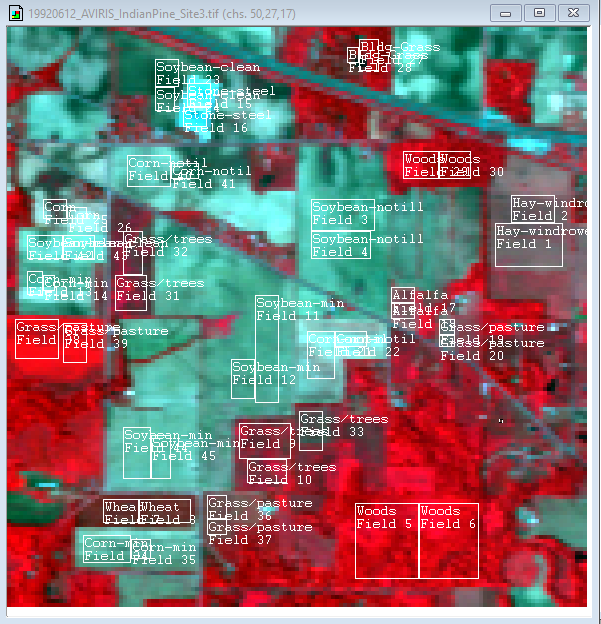
\includegraphics[height=8.0cm]{imgs/Dataset.png}
	\end{center}
	\caption{AVIRIS 92AV3C dataset for experiment}
	\label{fig:AVIRIS 92AV3C dataset for experiment}
\end{figure}

\begin{figure}[H]
	\begin{center}
		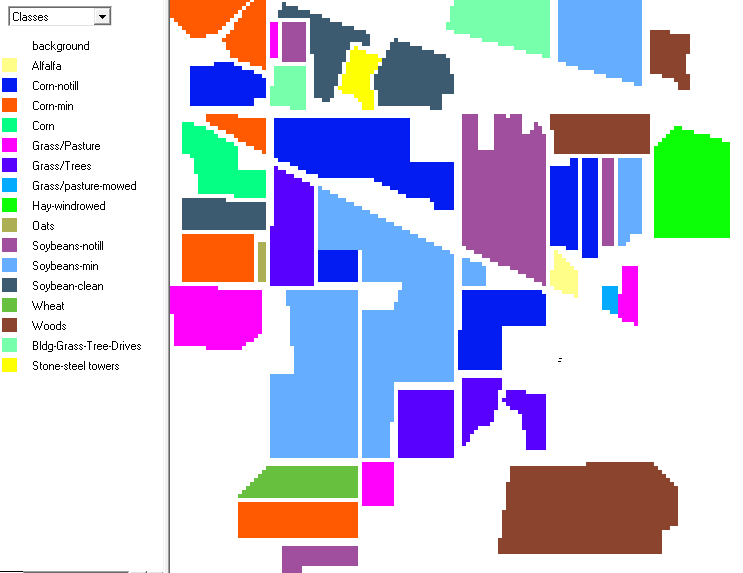
\includegraphics[height=8.0cm]{imgs/Ground.png}
	\end{center}
	\caption{Ground truth of AVIRIS 92AV3C dataset}
	\label{fig:Ground truth of AVIRIS 92AV3C dataset}
\end{figure}

\subsection{Feature Extraction Result}
The first few PCA images  have 99\% of the total variance of the input data set. The first component is the brightest and sharpest.
Fig. 1 shows few PCA images. 
\begin{figure}[H]
	\begin{center}
		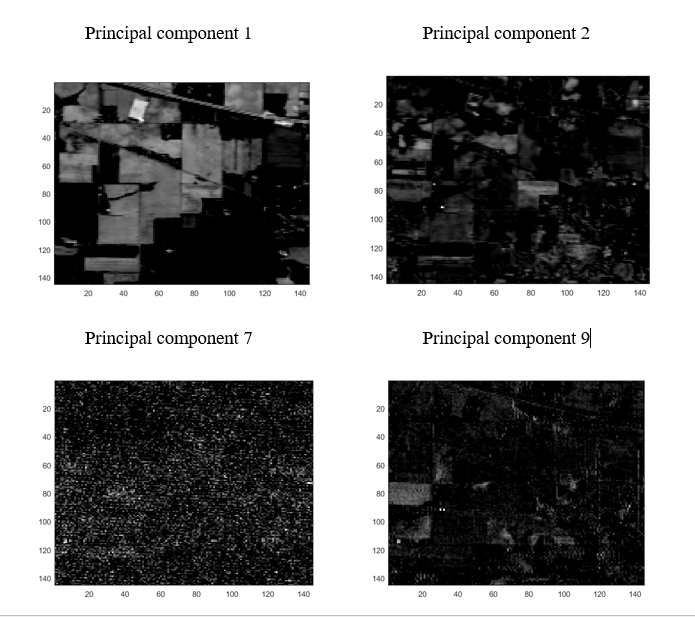
\includegraphics[height=15.0cm]{imgs/PC.png}
	\end{center}
	\caption{PCA image 1, 2, 7 and 9.}
	\label{fig:Some principal components}
\end{figure}

\noindent It is not always true that higher the variance higher the information. In Fig. 1, it is visually shown that the PCA image 7 has high variance but less spatial information than PCA image 9.
%\noindent In this research, at first the dimensions of the dataset is reduced from 220 using PCA. Here first few component contains most of the variation of the dataset. Figure 4.3 shows few components after applying PCA to the original AVIRIS 92AV3C dataset. First component is the most informative than second and so on. But PCA considers only the global variable of the dataset therefore some components may have more variance but less information for some specific class. Principal component 7 and principal component 9 is an example of this problem of PCA.
%\begin{figure}[H]
%	\begin{center}
%		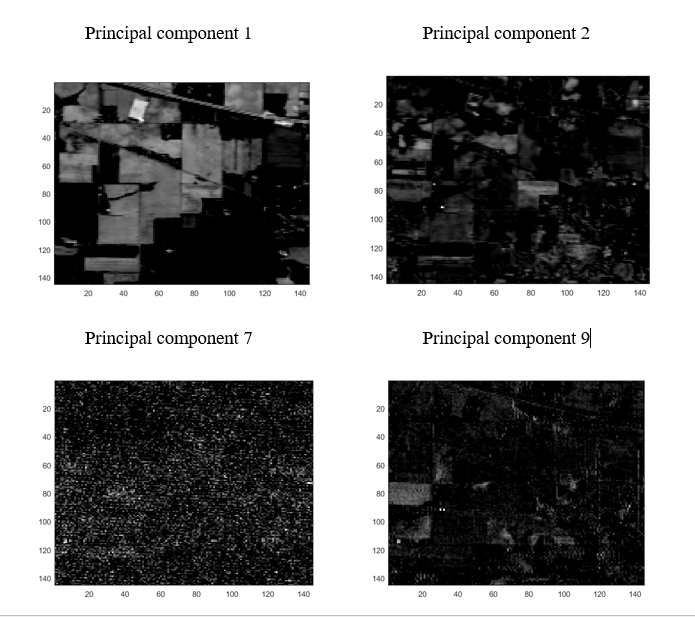
\includegraphics[height=15.0cm]{imgs/PC.png}
%	\end{center}
%	\caption{Some principal components}
%	\label{fig:Some principal components}
%\end{figure}
\begin{figure}[H]
	\begin{center}
		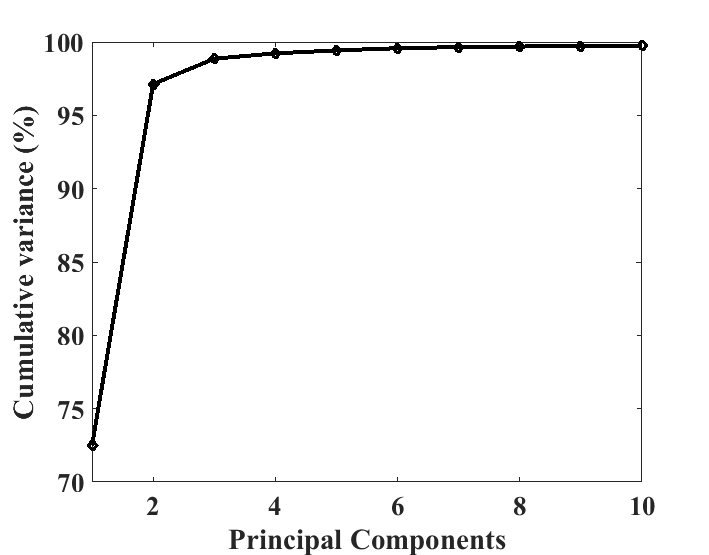
\includegraphics[height=10.0cm]{imgs/Var.png}
	\end{center}
	\caption{Cumulative variance of bands obtained via PCA}
	\label{fig:Cumulative variance of bands obtained via PCA}
\end{figure}
\noindent Figure 4.4 represents the cumulative relations between variance and each component. Here we can see than first 8 components of PCA has contain 99.69\% variations of the dataset.
\subsection{nMI Based Feature Selection Result}
%\subsubsection{Original Dataset Plus nMI Approach}
%\begin{table}[H]
%	\caption{Selected features with Org+NMI}
%	\begin{center}
%		\begin{tabular}{|c|c|}
%			\hline
%			Method & Order of selected features\\ \hline
%			Org+NMI & Band: 27,1,167,3,139,14,2,8\\ \hline
%		\end{tabular}
%	\end{center}
%	\label{tab:Selected features with Org+NMI}
%\end{table}
%\begin{figure}[H]
%	\begin{center}
%		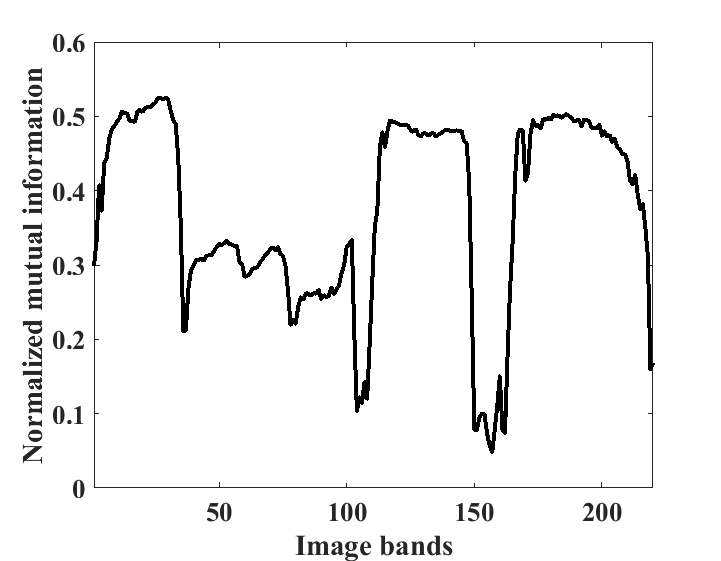
\includegraphics[height=7.0cm]{imgs/OrgNmi.png}
%	\end{center}
%	\caption{Normalized mutual information between class labels and original bands}
%	\label{fig:Normalized mutual information between class labels and original bands}
%\end{figure}
%\subsubsection{PCA Dataset Plus nMI Approach}
%\begin{table}[H]
%	\caption{Selected features with PCA+NMI}
%	\begin{center}
%		\begin{tabular}{|c|c|}
%			\hline
%			Method & Order of selected features\\ \hline
%			Org+NMI & PC: 1,4,3,5,6,9,15,2\\ \hline
%		\end{tabular}
%	\end{center}
%	\label{tab:Selected features with PCA+NMI}
%\end{table}
%\begin{figure}[H]
%	\begin{center}
%		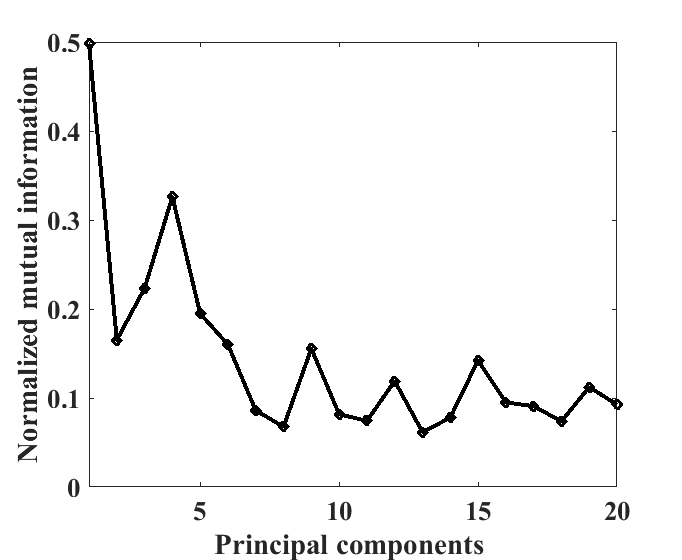
\includegraphics[height=8.0cm]{imgs/nmi.png}
%	\end{center}
%	\caption{Normalized mutual information between class labels and PC1-PC20}
%	\label{fig:Normalized mutual information between class labels and PC1-PC20}
%\end{figure}

To address the limitation of PCA, feature selection method is used. Normalized mutual information as selection technique is applied to overcome the problem of PCA. Table-4.1 shows selected features applying NMI over original bands and Table-4.2 shows the selected features applying NMI over PCA images. It is seen that the PC9 is selected but not PC7. 
\begin{table}[H]
	\caption{Selected features with Org+NMI}
	\begin{center}
		\begin{tabular}{|c|c|}
			\hline
			Method & Order of selected features\\ \hline
			Org+NMI & Band: 27,1,167,3,139,14,2,8\\ \hline
		\end{tabular}
	\end{center}
	\label{tab:Selected features with Org+NMI}
\end{table}
\begin{figure}[H]
	\begin{center}
		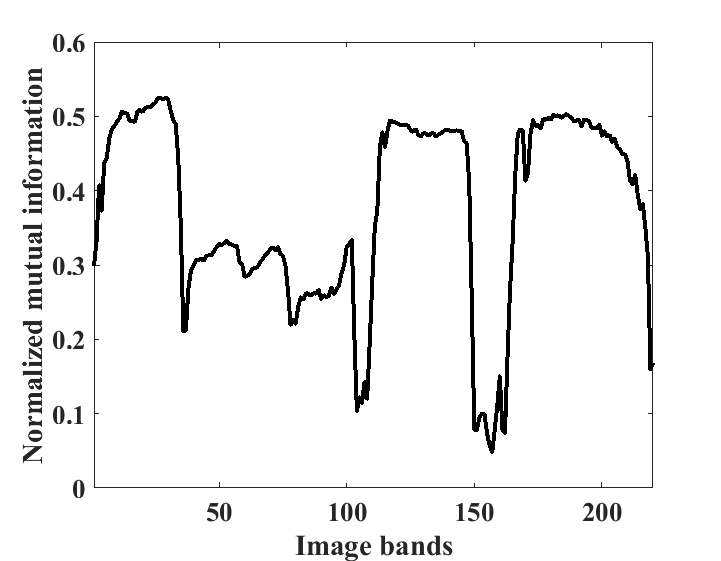
\includegraphics[height=10.0cm]{imgs/OrgNmi.png}
	\end{center}
	\caption{Normalized mutual information between class labels and original bands}
	\label{fig:Normalized mutual information between class labels and original bands}
\end{figure}

\noindent Fig. 4.5 shows the NMI between class labels and original data bands. The higher the NMI value of a band, the band is more important for the classification. Fig. 4.6 represents NMI between class labels and first 20 principal components. Therefore, in PCA+NMI, principal components are selected based on high value of NMI. 

\begin{table}[H]
	\caption{Selected features with PCA+NMI}
	\begin{center}
		\begin{tabular}{|c|c|}
			\hline
			Method & Order of selected features\\ \hline
			PCA+NMI & PC: 1,4,3,5,9,6,2,15\\ \hline
		\end{tabular}
	\end{center}
	\label{tab:Selected features with PCA+NMI}
\end{table}

\begin{figure}[H]
	\begin{center}
		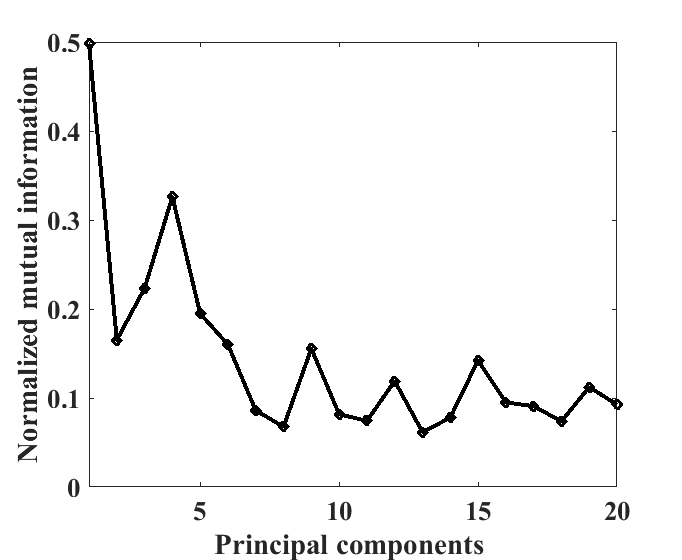
\includegraphics[height=10.0cm]{imgs/nmi.png}
	\end{center}
	\caption{Normalized mutual information between class labels and PC1-PC20}
	\label{fig:Normalized mutual information between class labels and PC1-PC20}
\end{figure}

\subsection{Proposed Method Result}
In this experiment, we proposed a target class oriented feature selection method (TCOSD) using NMI measure for maximizing the relevance of the selected subspace.The objective is to show that the target class oriented feature selection is more effective than the traditional feature selection while considering all the classes together. The proposed method manages this situation by considering one class as target at a time and the remaining as the background. Table-4.3 shows the selected features for each target class. 
\begin{table}[H]
	\caption{Selected features for each target class with proposed method (TCOSD)}
	\begin{center}
		\begin{tabular}{|c|l|}
			\hline
			Target class & Order of selected features\\ \hline
			Hay-windrowed & PC: 4,1,17,5,12,3,16,2\\ \hline
			Soybean-notil & PC: 1,17,16,11,20,14,13,3\\ \hline
			Woods & PC: 1,16,17,3,15,11,5,20\\ \hline
			Wheat & PC: 6,19,17,3,12,16,11,5\\ \hline
			Grass/trees & PC: 4,9,5,6,16,17,2,1\\ \hline
			Soybean-min & PC: 1,17,16,3,5,12,11,9\\ \hline
			Corn-min & PC: 1,17,16,5,11,3,20,19\\ \hline
			Stone-steel & PC: 3,4,1,17,16,10,5,11\\ \hline
			Alfalfa & PC: 4,17,15,20,3,16,6,12\\ \hline
			Grass/Pasture & PC: 9,3,17,6,16,11,1,15\\ \hline
			Corn-notill & PC: 1,17,2,16,11,18,20,19\\ \hline
			Soybean-clean & PC: 1,15,17,3,16,20,12,11\\ \hline
			Corn & PC: 1,19,17,16,18,8,11,3\\ \hline
			Bldg-Grass & PC: 15,16,17,3,18,11,19,4\\ \hline
		\end{tabular}
	\end{center}
	\label{tab:Selected features for each target class with proposed method (TCOSD)}
\end{table}


\section{Classification Results}
%\begin{table}[H]
%	\caption{Details of the training and test samples}
%	\begin{center}
%		\begin{tabular}{|c|c|c|}
%			\hline
%			Class name & Train & Test\\ \hline
%			Hay-windrowed & 187 & 77\\ \hline
%			Soybean-notil & 128 & 105\\ \hline
%			Woods & 367 & 341\\ \hline
%			Wheat & 54 & 78\\ \hline
%			Grass/trees & 249 & 115\\ \hline
%			Soybean-min & 253 & 115\\ \hline
%			Corn-min & 253 & 115\\ \hline
%			Stone-steel & 36 & 30\\ \hline
%			Alfalfa & 24 & 24\\ \hline
%			Grass/Pasture & 156 & 92\\ \hline
%			Corn-notill & 172 & 60\\ \hline
%			Soybean-clean & 96 & 78\\ \hline
%			Corn & 30 & 15\\ \hline
%			Bldg-Grass & 40 & 12\\ \hline
%			Total & 1900 & 1179\\ \hline
%		\end{tabular}
%	\end{center}
%	\label{tab:Details of the training and test samples}
%\end{table}
%
%\begin{table}[H]
%	\caption{Details of parameter for KSVM(RBF kernel)}
%	\begin{center}
%		\begin{tabular}{|c|c|c|}
%			\hline
%			Method & C & $\gamma$ \\ \hline
%			Org+NMI & 10 & 2.44 \\ \hline
%			PCA & 9 & 5.72 \\ \hline
%			PCA+NMI & 10 & 6\\ \hline
%			TCO+PCA+NMI & 5 & 0.75\\ \hline
%		\end{tabular}
%	\end{center}
%	\label{tab:Details of parameter for KSVM(RBF kernel)}
%\end{table}
%
%\begin{table}[H]
%	\caption{Classification result for 8 features}
%	\begin{center}
%		\begin{tabular}{|c|c|}
%			\hline
%			Method & Classification Result\\ \hline
%			Org+NMI & 72.26\%\\ \hline
%			PCA & 89.05\%\\ \hline
%			PCA+NMI & 92.79\%\\ \hline
%			TCO+PCA+NMI & 96.57\%\\ \hline
%		\end{tabular}
%	\end{center}
%	\label{tab:Classification result for 8 features}
%\end{table}
%
%%\begin{figure}[H]
%%	\begin{center}
%%		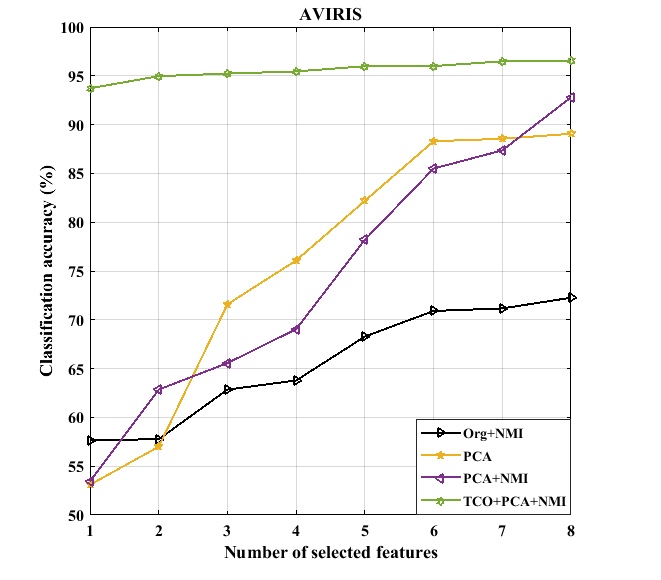
\includegraphics[height=10.0cm]{imgs/4MethodsAc.png}
%%	\end{center}
%%	\caption{Classification accuracy of AVIRIS 92AV3c data}
%%	\label{fig:Classification accuracy of AVIRIS 92AV3c data}
%%\end{figure}

The hyperspectral image named 92AV3C which was captured over the indian pine test site in Northwestern indiana by the NASA AVIRIS sensor\cite{30} is used as the input data set. It has 220 image bands which contains 145$\times$145 pixels. The ground truth available have sixteen classes. In the experiment, 14 classes are used, because the oats and another class are too small. Details training and testing samples of AVIRIS 92AV3C data set is shown in Table 4.4.
\begin{table}[H]
	\caption{Details of the train and test samples}
	\begin{center}
		\begin{tabular}{|l|l|l|}
			\hline
			Class name & Train & Test\\ \hline
			Hay-windrowed & 187 & 77\\ \hline
			Soybean-notil & 128 & 105\\ \hline
			Woods & 367 & 341\\ \hline
			Wheat & 54 & 78\\ \hline
			Grass/trees & 249 & 115\\ \hline
			Soybean-min & 253 & 115\\ \hline
			Corn-min & 253 & 115\\ \hline
			Stone-steel & 36 & 30\\ \hline
			Alfalfa & 24 & 24\\ \hline
			Grass/Pasture & 156 & 92\\ \hline
			Corn-notill & 172 & 60\\ \hline
			Soybean-clean & 96 & 78\\ \hline
			Corn & 30 & 15\\ \hline
			Bldg-Grass & 40 & 12\\ \hline
			Total & 1900 & 1179\\ \hline
		\end{tabular}
	\end{center}
	\label{tab:Details of the train and test samples}
\end{table}

\noindent The Selected features is applied to a KSVM classifier. A comparison of the classification accuracy is presented in Table-4.5 and it can be seen that the proposed method outperforms the baseline approaches.
\begin{table}[H]
	\caption{Details of parameter for KSVM(RBF kernel)}
	\begin{center}
		\begin{tabular}{|c|c|c|}
			\hline
			Method & C & $\gamma$ \\ \hline
			Org+NMI & 10 & 2.44 \\ \hline
			PCA & 19 & 2.40 \\ \hline
			PCA+NMI & 16 & 0.7\\ \hline
			TCOSD & 5 & 0.75\\ \hline
		\end{tabular}
	\end{center}
	\label{tab:Details of parameter for KSVM(RBF kernel)}
\end{table}
\noindent The kernel hyperparameter such as the best cost C and kernel width $\gamma$ are calculated using 10 fold cross-validation\cite{29}. Table-4.4 shows kernel hyperparameter used in this experiment.
\begin{table}[H]
	\caption{Classification result for 8 features}
	\begin{center}
		\begin{tabular}{|c|c|}
			\hline
			Method & Classification Result\\ \hline
			Org+NMI & 72.26\%\\ \hline
			PCA & 89.90\%\\ \hline
			PCA+NMI & 93.12\%\\ \hline
			TCOSD& 96.57\%\\ \hline
		\end{tabular}
	\end{center}
	\label{tab:Classification result for 10 features}
\end{table}
\noindent Fig. 4.7 shows a visualization of comparison among the proposed approach and some standard approach studied when the classification accuracy is determined by adding the features progressively.\\
\begin{figure}[H]
	\begin{center}
		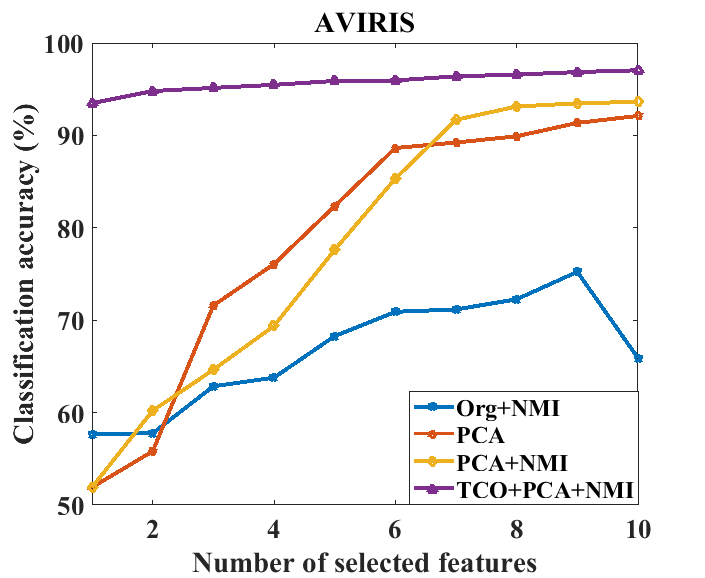
\includegraphics[height=10.0cm]{imgs/Res.png}
	\end{center}
	\caption{Classification accuracy of AVIRIS 92AV3C data}
	\label{fig:Classification accuracy of AVIRIS 92AV3C data}
\end{figure}

\end{document}